\documentclass[10pt,oneside]{article}
\usepackage[T1]{fontenc}
\usepackage[utf8]{inputenc}
%\usepackage[latin1]{inputenc}
\DeclareUnicodeCharacter{00A0}{ }
% \usepackage{lmodern}
%\usepackage[adobe-utopia,uppercase=upright,greeklowercase=upright]{mathdesign}
\usepackage[adobe-utopia]{mathdesign}
%\usepackage{minionpro}
% \usepackage{pifont}
% \usepackage{amssymb}
\usepackage{amsmath}
\usepackage[francais]{babel}
% \usepackage[francais]{varioref}
\usepackage[dvips]{graphicx}
\usepackage{here}
\usepackage{framed}
\usepackage[normalem]{ulem}
\usepackage{fancyhdr}
\usepackage{titlesec}
\usepackage{vmargin}
\usepackage{longtable}

\usepackage{amsmath}

\usepackage{ifthen}
%\usepackage[•]{caption}

%\usepackage{epsfig}
\usepackage{subfig}

\usepackage{multirow}
\usepackage{multicol} % Portions de texte en colonnes
\usepackage{flafter}%floatants après la référence



\usepackage{color}
\usepackage{colortbl}


\definecolor{gris25}{gray}{0.75}
\definecolor{bleu}{RGB}{18,33,98}
\definecolor{bleuf}{RGB}{42,94,171}
\definecolor{bleuc}{RGB}{231,239,247}
\definecolor{rougef}{RGB}{185,18,27}
\definecolor{rougec}{RGB}{255,230,231}
\definecolor{vertf}{RGB}{103,126,82}
\definecolor{vertc}{RGB}{220,255,191}
\definecolor{violetf}{RGB}{112,48,160}
\definecolor{violetc}{RGB}{230,224,236}
\definecolor{jaunec}{RGB}{220,255,191}

\newenvironment{sci}[1][\hsize]%
{%
    \def\FrameCommand%
    {%
%\rotatebox{90}{\textit{\textsf{Scilab}}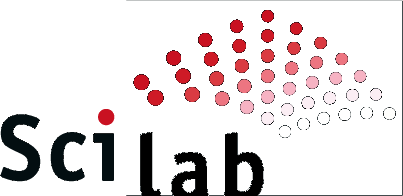
\includegraphics[height=.8cm]{png/logo_scilab}} 
\rotatebox{90}{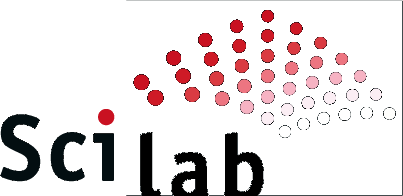
\includegraphics[height=.6cm]{png/logo_scilab}} 
        {\color{violetf}\vrule width 3pt}%
        \hspace{0pt}%must no space.
        \fboxsep=\FrameSep\colorbox{violetc}%
    }%
    \MakeFramed{\hsize #1 \advance\hsize-\width\FrameRestore}%
}%
{\endMakeFramed}%

\newenvironment{pseudo}[1][\hsize]%
{%
    \def\FrameCommand%
    {%
\rotatebox{90}{\textit{\textsf{Pseudo Code}}} 
        {\color{violetf}\vrule width 3pt}%
        \hspace{0pt}%must no space.
        \fboxsep=\FrameSep\colorbox{violetc}%
    }%
    \MakeFramed{\hsize #1 \advance\hsize-\width\FrameRestore}%
}%
{\endMakeFramed}%

\newenvironment{py}[1][\hsize]%
{%
    \def\FrameCommand%
    {%
%\rotatebox{90}{\textit{\textsf{Python}}} 
\rotatebox{90}{
\includegraphics[height=.6cm]{png/logo_python}} 
        {\color{violetf}\vrule width 3pt}%
        \hspace{0pt}%must no space.
        \fboxsep=\FrameSep\colorbox{violetc}%
    }%
    \MakeFramed{\hsize #1 \advance\hsize-\width\FrameRestore}%
}%
{\endMakeFramed}%


\newenvironment{term}[1][\hsize]%
{%
    \def\FrameCommand%
    {%
\rotatebox{90}{\textit{\textsf{Terminal}}} 
        {\color{violetf}\vrule width 3pt}%
        \hspace{0pt}%must no space.
        \fboxsep=\FrameSep\colorbox{violetc}%
    }%
    \MakeFramed{\hsize #1 \advance\hsize-\width\FrameRestore}%
}%
{\endMakeFramed}%


\newenvironment{rem}[1][\hsize]%
{%
    \def\FrameCommand
    {%
\rotatebox{90}{\textit{\textsf{Remarque}}} 
        {\color{bleuf}\vrule width 3pt}%
        \hspace{0pt}%must no space.
        \fboxsep=\FrameSep\colorbox{bleuc}%
    }%
    \MakeFramed{\hsize#1\advance\hsize-\width\FrameRestore}%
}%
{\endMakeFramed}%


\newenvironment{savoir}[1][\hsize]%
{%
    \def\FrameCommand
    {%
\rotatebox{90}{\textit{\textsf{Savoir}}} 
        {\color{bleuf}\vrule width 3pt}%
        \hspace{0pt}%must no space.
        \fboxsep=\FrameSep\colorbox{bleuc}%
    }%
    \MakeFramed{\hsize#1\advance\hsize-\width\FrameRestore}%
}%
{\endMakeFramed}%

\newenvironment{objectif}[1][\hsize]%
{%
    \def\FrameCommand
    {%
\rotatebox{90}{\textit{\textsf{Objectif}}} 
        {\color{rougef}\vrule width 3pt}%
        \hspace{0pt}%must no space.
        \fboxsep=\FrameSep\colorbox{rougec}%
    }%
    \MakeFramed{\hsize#1\advance\hsize-\width\FrameRestore}%
}%
{\endMakeFramed}%

\newenvironment{prob}[1][\hsize]%
{%
    \def\FrameCommand%
    {%
\rotatebox{90}{\textit{\textsf{ Problématique}}} 
        {\color{rougef}\vrule width 3pt}%
        \hspace{0pt}%must no space.
        \fboxsep=\FrameSep\colorbox{rougec}%
    }%
    \MakeFramed{\hsize#1\advance\hsize-\width\FrameRestore}%
}%
{\endMakeFramed}%

\newenvironment{obj}[1][\hsize]%
{%
    \def\FrameCommand%
    {%
\rotatebox{90}{\textit{\textsf{ $\;$}}} 
        {\color{rougef}\vrule width 3pt}%
        \hspace{0pt}%must no space.
        \fboxsep=\FrameSep\colorbox{rougec}%
    }%
    \MakeFramed{\hsize#1\advance\hsize-\width\FrameRestore}%
}%
{\endMakeFramed}%

\newenvironment{defi}[1][\hsize]%
{%
    \def\FrameCommand%
    {%
\rotatebox{90}{\textit{\textsf{Définition\\}}} 
        {\color{bleuf}\vrule width 3pt}%
        \hspace{0pt}%must no space.
        \fboxsep=\FrameSep\colorbox{bleuc}%
    }%
    \MakeFramed{\hsize#1\advance\hsize-\width\FrameRestore}%
}%
{\endMakeFramed}%


\newenvironment{demo}[1][\hsize]%
{%
    \def\FrameCommand%
    {%
\rotatebox{90}{\textit{\textsf{Démonstration\\}}} 
        {\color{bleuf}\vrule width 3pt}%
        \hspace{0pt}%must no space.
        \fboxsep=\FrameSep\colorbox{bleuc}%
    }%
    \MakeFramed{\hsize#1\advance\hsize-\width\FrameRestore}%
}%
{\endMakeFramed}%


\newenvironment{hypo}[1][\hsize]%
{%
    \def\FrameCommand%
    {%
\rotatebox{90}{\textit{\textsf{Hypothèse\\}}} 
        {\color{bleuf}\vrule width 3pt}%
        \hspace{0pt}%must no space.
        \fboxsep=\FrameSep\colorbox{bleuc}%
    }%
    \MakeFramed{\hsize#1\advance\hsize-\width\FrameRestore}%
}%
{\endMakeFramed}%


\newenvironment{prop}[1][\hsize]%
{%
    \def\FrameCommand%
    {%
\rotatebox{90}{\textit{\textsf{Propriété\\}}} 
        {\color{bleuf}\vrule width 3pt}%
        \hspace{0pt}%must no space.
        \fboxsep=\FrameSep\colorbox{bleuc}%
    }%
    \MakeFramed{\hsize#1\advance\hsize-\width\FrameRestore}%
}%
{\endMakeFramed}%

\newenvironment{props}[1][\hsize]%
{%
    \def\FrameCommand%
    {%
\rotatebox{90}{\textit{\textsf{Propriétés\\}}} 
        {\color{bleuf}\vrule width 3pt}%
        \hspace{0pt}%must no space.
        \fboxsep=\FrameSep\colorbox{bleuc}%
    }%
    \MakeFramed{\hsize#1\advance\hsize-\width\FrameRestore}%
}%
{\endMakeFramed}%

\newenvironment{exemple}[1][\hsize]%
{%
    \def\FrameCommand%
    {%
\rotatebox{90}{\textit{\textsf{Exemple\\}}} 
        {\color{vertf}\vrule width 3pt}%
        \hspace{0pt}%must no space.
        \fboxsep=\FrameSep\colorbox{vertc}%
    }%
    \MakeFramed{\hsize#1\advance\hsize-\width\FrameRestore}%
}%
{\endMakeFramed}%

\newenvironment{exercice}[1][\hsize]%
{%
    \def\FrameCommand%
    {%
\rotatebox{90}{\textit{\textsf{Exercice\\}}} 
        {\color{vertf}\vrule width 3pt}%
        \hspace{0pt}%must no space.
        \fboxsep=\FrameSep\colorbox{vertc}%
    }%
    \MakeFramed{\hsize#1\advance\hsize-\width\FrameRestore}%
}%
{\endMakeFramed}%

\newenvironment{Support}[1][\hsize]%
{%
    \def\FrameCommand%
    {%
\rotatebox{90}{\textit{\textsf{Support de cours\\}}} 
        {\color{vertf}\vrule width 3pt}%
        \hspace{0pt}%must no space.
        \fboxsep=\FrameSep\colorbox{jaunec}%
    }%
    \MakeFramed{\hsize#1\advance\hsize-\width\FrameRestore}%
}%
{\endMakeFramed}%

\newenvironment{resultat}[1][\hsize]%
{%
    \def\FrameCommand%
    {%
\rotatebox{90}{\textit{\textsf{Résultat\\}}} 
        {\color{rougef}\vrule width 3pt}%
        \hspace{0pt}%must no space.
        \fboxsep=\FrameSep\colorbox{rougec}%
    }%
    \MakeFramed{\hsize#1\advance\hsize-\width\FrameRestore}%
}%
{\endMakeFramed}%

\newenvironment{methode}[1][\hsize]%
{%
    \def\FrameCommand%
    {%
\rotatebox{90}{\textit{\textsf{Méthode\\}}} 
        {\color{rougef}\vrule width 3pt}%
        \hspace{0pt}%must no space.
        \fboxsep=\FrameSep\colorbox{rougec}%
    }%
    \MakeFramed{\hsize#1\advance\hsize-\width\FrameRestore}%
}%
{\endMakeFramed}%

\newenvironment{theo}[1][\hsize]%
{%
    \def\FrameCommand%
    {%
\rotatebox{90}{\textit{\textsf{Théorème\\}}} 
        {\color{rougef}\vrule width 3pt}%
        \hspace{0pt}%must no space.
        \fboxsep=\FrameSep\colorbox{rougec}%
    }%
    \MakeFramed{\hsize#1\advance\hsize-\width\FrameRestore}%
}%
{\endMakeFramed}%

\newenvironment{warn}[1][\hsize]%
{%
    \def\FrameCommand%
    {%
\rotatebox{90}{\textit{\textsf{Attention\\}}} 
        {\color{rougef}\vrule width 3pt}%
        \hspace{0pt}%must no space.
        \fboxsep=\FrameSep\colorbox{rougec}%
    }%
    \MakeFramed{\hsize#1\advance\hsize-\width\FrameRestore}%
}%
{\endMakeFramed}%

% \usepackage{pstricks}
%\usepackage{minitoc}
% \setcounter{minitocdepth}{4}

\setcounter{tocdepth}{2}

% \mtcselectlanguage{french} 

%\usepackage{draftcopy}% "Brouillon"
% \usepackage{floatflt}
\usepackage{psfrag}
%\usepackage{listings} % Permet d'insérer du code de programmation
\renewcommand{\baselinestretch}{1.2}

% Changer la numérotation des figures :
% ------------------------------------
% \makeatletter
% \renewcommand{\thefigure}{\ifnum \c@section>\z@ \thesection.\fi
%  \@arabic\c@figure}
% \@addtoreset{figure}{section}
% \makeatother
 


%%%%%%%%%%%%
% Définition des vecteurs %
%%%%%%%%%%%%
 \newcommand{\vect}[1]{\overrightarrow{#1}}

%%%%%%%%%%%%
% Définition des torseusr %
%%%%%%%%%%%%

 \newcommand{\torseur}[1]{%
\left\{{#1}\right\}
}

\newcommand{\torseurcin}[3]{%
\left\{\mathcal{#1} \left(#2/#3 \right) \right\}
}

\newcommand{\torseurstat}[3]{%
\left\{\mathcal{#1} \left(#2\rightarrow #3 \right) \right\}
}

 \newcommand{\torseurc}[8]{%
%\left\{#1 \right\}=
\left\{
{#1}
\right\}
 = 
\left\{%
\begin{array}{cc}%
{#2} & {#5}\\%
{#3} & {#6}\\%
{#4} & {#7}\\%
\end{array}%
\right\}_{#8}%
}

 \newcommand{\torseurcol}[7]{
\left\{%
\begin{array}{cc}%
{#1} & {#4}\\%
{#2} & {#5}\\%
{#3} & {#6}\\%
\end{array}%
\right\}_{#7}%
}

 \newcommand{\torseurl}[3]{%
%\left\{\mathcal{#1}\right\}_{#2}=%
\left\{%
\begin{array}{l}%
{#1} \\%
{#2} %
\end{array}%
\right\}_{#3}%
}

 \newcommand{\vectv}[3]{%
\vect{V\left( {#1} \in {#2}/{#3}\right)}
}


\newcommand{\vectf}[2]{%
\vect{R\left( {#1} \rightarrow {#2}\right)}
}

\newcommand{\vectm}[3]{%
\vect{\mathcal{M}\left( {#1}, {#2} \rightarrow {#3}\right)}
}


 \newcommand{\vectg}[3]{%
\vect{\Gamma \left( {#1} \in {#2}/{#3}\right)}
}

 \newcommand{\vecto}[2]{%
\vect{\Omega\left( {#1}/{#2}\right)}
}
% }$$\left\{\mathcal{#1} \right\}_{#2} =%
% \left\{%
% \begin{array}{c}%
%  #3 \\%
%  #4 %
% \end{array}%
% \right\}_{#5}}

%  ------------------------------------------
% | Modification du formatage des sections : | 
%  ------------------------------------------

% Grands titres :
% ---------------

\newcommand{\titre}[1]{%
\begin{center}
      \bigskip
      \rule{\textwidth}{1pt}
      \par\vspace{0.1cm}
      
      \textbf{\large #1}
      \par\rule{\textwidth}{1pt}
    \end{center}
    \bigskip
  }

% Supprime le numéro du chapitre dans la numérotation des sections:
% -----------------------------------------------------------------
\makeatletter
\renewcommand{\thesection}{\@arabic\c@section}
\makeatother


% \titleformat{\chapter}[display]
% {\normalfont\Large\filcenter}
% {}
% {1pc}
% {\titlerule[1pt]
%   \vspace{1pc}%
%   \Huge}[\vspace{1ex}%
% \titlerule]


%%%% Chapitres Comme PY Pechard %%%%%%%%%
% numéro du chapitre
\DeclareFixedFont{\chapnumfont}{OT1}{phv}{b}{n}{80pt}
% pour le mot « Chapitre »
\DeclareFixedFont{\chapchapfont}{OT1}{phv}{m}{it}{40pt}
% pour le titre
\DeclareFixedFont{\chaptitfont}{T1}{phv}{b}{n}{25pt}

\definecolor{gris}{gray}{0.75}
\titleformat{\chapter}[display]%
	{\sffamily}%
	{\filleft\chapchapfont\color{gris}\chaptertitlename\
	\\
	\vspace{12pt}
	\chapnumfont\thechapter}%
	{16pt}%
	{\filleft\chaptitfont}%
	[\vspace{6pt}\titlerule\titlerule\titlerule]

%%%%  Fin Chapitres Comme PY Pechard %%%%%%%%%


% Section, subsection, subsubsection sans serifs :
% % ----------------------------------------------

% \makeatletter
% \renewcommand{\section}{\@startsection{section}{0}{0mm}%
% {\baselineskip}{.3\baselineskip}%
% {\normalfont\sffamily\Large\textbf}}%
% \makeatother

\makeatletter
\renewcommand{\@seccntformat}[1]{{\textcolor{bleu}{\csname
the#1\endcsname}\hspace{0.5em}}}
\makeatother

\makeatletter
\renewcommand{\section}{\@startsection{section}{1}{\z@}%
                       {-4ex \@plus -1ex \@minus -.4ex}%
                       {1ex \@plus.2ex }%
                       {\normalfont\Large\sffamily\bfseries}}%
\makeatother
 
\makeatletter
\renewcommand{\subsection}{\@startsection {subsection}{2}{\z@}
                          {-3ex \@plus -0.1ex \@minus -.4ex}%
                          {0.5ex \@plus.2ex }%
                          {\normalfont\large\sffamily\bfseries}}
\makeatother
 
\makeatletter
\renewcommand{\subsubsection}{\@startsection {subsubsection}{3}{\z@}
                          {-2ex \@plus -0.1ex \@minus -.2ex}%
                          {0.2ex \@plus.2ex }%
                          {\normalfont\large\sffamily\bfseries}}
\makeatother
 
\makeatletter             
\renewcommand{\paragraph}{\@startsection{paragraph}{4}{\z@}%
                                    {-2ex \@plus-.2ex \@minus .2ex}%
                                    {0.1ex}%               
{\normalfont\sffamily\bfseries}}
\makeatother
 
 
\makeatletter             
\renewcommand{\subparagraph}{\@startsection{subparagraph}{5}{\z@}%
                                    {-2ex \@plus-.2ex \@minus .2ex}%
                                    {0ex}%               
{\normalfont\bfseries Question }}
\makeatother
\renewcommand{\thesubparagraph}{\arabic{subparagraph}} 
\makeatletter


\renewcommand{\thesubparagraph}{\arabic{subparagraph}} 

% \makeatletter
% \renewcommand{\subsection}{\@startsection{subsection}{1}{2mm}%
% {\baselineskip}{.3\baselineskip}%
% {\normalfont\sffamily\large\textbf}}%
% \makeatother
% 
% \makeatletter
% \renewcommand{\subsubsection}{\@startsection{subsubsection}{2}{4mm}%
% {\baselineskip}{.15\baselineskip}%
% {\normalfont\sffamily\large\textbf}}%
% \makeatother
% 
% \makeatletter
% \renewcommand{\paragraph}{\@startsection{paragraph}{3}{6mm}%
% {\baselineskip}{.15\baselineskip}%
% {\normalfont\sffamily\large\textbf}}%
% \makeatother
 
\setcounter{secnumdepth}{5}


%  --------
% | Marges |
%  --------


% \setmarginsrb{2.5cm}{1.5cm}{2.5cm}{2cm}{1cm}{1cm}{1cm}{1cm}
\setmarginsrb{1.5cm}{1cm}{1cm}{1.5cm}{1cm}{1cm}{1cm}{1cm}

% Changer les marges localement :
% -----------------------------
\newenvironment{changemargin}[2]{\begin{list}{}{%
\setlength{\topsep}{0pt}%
\setlength{\leftmargin}{0pt}%
\setlength{\rightmargin}{0pt}%
\setlength{\listparindent}{\parindent}%
\setlength{\itemindent}{\parindent}%
\setlength{\parsep}{0pt plus 1pt}%
\addtolength{\leftmargin}{#1}%
\addtolength{\rightmargin}{#2}%
}\item }{\end{list}}



\usepackage{pst-solides3d}
\usepackage{titletoc}
\titlecontents{chapter}[+3pc]
  {\addvspace{10pt}\sffamily\bfseries}
{\contentslabel[{\pscirclebox[fillstyle=solid,fillcolor=gray!25,
linecolor=gray!25,framesep=4pt]{\textcolor{white}{\thecontentslabel}}}]{2.5pc}}
  {}
  {\dotfill \normalfont\thecontentspage\ }

\titlecontents{section}[3pc]
  {\addvspace{2pt}\sffamily}
  {\contentslabel[\thecontentslabel]{1.8pc}}
  {}
  {\dotfill \normalfont\thecontentspage\ }

\titlecontents{subsection}[5pc]
  {\addvspace{2pt}\sffamily}
  {\contentslabel[\thecontentslabel]{1.8pc}}
  {}
  {\dotfill \normalfont\thecontentspage\ }

\titlecontents{subsubsection}[8pc]
  {\addvspace{2pt}\sffamily}
  {\contentslabel[\thecontentslabel]{3pc}}
  {}
  {\dotfill \normalfont\thecontentspage\ }
%{\;\titlerule\;\normalfont\thecontentspage\ }

\titlecontents{paragraph}[9pc]
  {\addvspace{2pt}\sffamily}
  {\contentslabel[\thecontentslabel]{3.5pc}}
  {}
  {\dotfill \normalfont\thecontentspage\ }

%pour avoir l indentation dans minipage
\newdimen\oldparindent\oldparindent=\parindent

\makeatletter
\def\@iiiminipage#1#2[#3]#4{%
  \noindent
  \leavevmode
  \@pboxswfalse
  \setlength\@tempdima{#4}%
  \def\@mpargs{{#1}{#2}[#3]{#4}}%
  \setbox\@tempboxa\vbox\bgroup
    \color@begingroup
      \hsize\@tempdima
      \textwidth\hsize \columnwidth\hsize
      \@parboxrestore
      \parindent=\oldparindent
      \def\@mpfn{mpfootnote}\def\thempfn{\thempfootnote}\c@mpfootnote\z@
      \let\@footnotetext\@mpfootnotetext
      \let\@listdepth\@mplistdepth \@mplistdepth\z@
      \@minipagerestore
      \@setminipage}
\makeatother

%\usepackage{algorithm}
%\usepackage{algorithmic}
\usepackage[french]{algorithm2e}

\SetKwBlock{Fonction}{Début Fonction}{Fin Fonction}
\SetKwComment{Comment}{start}{end}
\SetKwFor{While}{Tant que}{Faire}{Fin tant que}
\SetKwIF{If}{ElseIf}{Else}{Si}{Alors}{Sinon si}{Sinon}{Fin si}
% Python sources

\usepackage{listings}
\lstloadlanguages{R}   % pour regler les pb d accent utf8 dans les codes
\lstset{language=R} % pour regler les pb d accent utf8 dans les codes

\usepackage{textcomp}
\usepackage{setspace}
%\usepackage{palatino}

%\usepackage{color}
\definecolor{Bleu}{rgb}{0.1,0.1,1.0}
\definecolor{Noir}{rgb}{0,0,0}
\definecolor{Grau}{rgb}{0.5,0.5,0.5}
\definecolor{DunkelGrau}{rgb}{0.15,0.15,0.15}
\definecolor{Hellbraun}{rgb}{0.5,0.25,0.0}
\definecolor{Magenta}{rgb}{1.0,0.0,1.0}
\definecolor{Gris}{gray}{0.5}
\definecolor{Vert}{rgb}{0,0.5,0}
\definecolor{SourceHintergrund}{rgb}{1,1.0,0.95}


%
\renewcommand{\lstlistlistingname}{Listings}
\renewcommand{\lstlistingname}{Listing}

\lstnewenvironment{python}[1][]{
\lstset{
numbers=left,
%escapeinside={\%*}{*)},
%inputencoding=utf8,   % pour regler les pb d accent utf8 dans les codes
%extendedchars=true,   % pour regler les pb d accent utf8 dans les codes
language=python,
basicstyle=\sffamily\footnotesize, 	
stringstyle=\color{red}, 
showstringspaces=false, 
alsoletter={1234567890},
otherkeywords={\ , \}, \{},
keywordstyle=\color{blue},
emph={access,and,break,class,continue,def,del,elif ,else,
except,exec,finally,for,from,global,if,import,in,i s,
lambda,not,or,pass,print,raise,return,try,while},
emphstyle=\color{black}\bfseries,
emph={[2]True, False, None, self},
emphstyle=[2]\color{green},
emph={[3]from, import, as},
emphstyle=[3]\color{blue},
upquote=true,
columns=flexible, % pour empecher d'avoir un espacement mono
morecomment=[s]{"""}{"""},
commentstyle=\color{Hellbraun}\slshape, 
%emph={[4]1, 2, 3, 4, 5, 6, 7, 8, 9, 0},
emphstyle=[4]\color{blue},
literate=*{:}{{\textcolor{blue}:}}{1}
{=}{{\textcolor{blue}=}}{1}
{-}{{\textcolor{blue}-}}{1}
{+}{{\textcolor{blue}+}}{1}
{*}{{\textcolor{blue}*}}{1}
{!}{{\textcolor{blue}!}}{1}
{(}{{\textcolor{blue}(}}{1}
{)}{{\textcolor{blue})}}{1}
{[}{{\textcolor{blue}[}}{1}
{]}{{\textcolor{blue}]}}{1}
{<}{{\textcolor{blue}<}}{1}
{>}{{\textcolor{blue}>}}{1}
{COMPLETER}{{\textcolor{red}COMPLETER}}{1},
literate=%
            {é}{{\'{e}}}1
            {è}{{\`{e}}}1
            {ê}{{\^{e}}}1
            {ë}{{\¨{e}}}1
            {û}{{\^{u}}}1
            {ù}{{\`{u}}}1
            {â}{{\^{a}}}1
            {à}{{\`{a}}}1
            {î}{{\^{i}}}1
            {ç}{{\c{c}}}1
            {Ç}{{\c{C}}}1
            {É}{{\'{E}}}1
            {Ê}{{\^{E}}}1
            {À}{{\`{A}}}1
            {Â}{{\^{A}}}1
            {Î}{{\^{I}}}1, % pour regler les pb d accent utf8 dans les codes
%framexleftmargin=1mm, framextopmargin=1mm, frame=shadowbox, rulesepcolor=\color{blue},#1
%backgroundcolor=\color{SourceHintergrund}, 
%framexleftmargin=1mm, framexrightmargin=1mm, framextopmargin=1mm, frame=single, framerule=1pt, rulecolor=\color{black},#1
}}{}



\lstnewenvironment{python2}[1][]{
\lstset{
%escapeinside={\%*}{*)},
%inputencoding=utf8,   % pour regler les pb d accent utf8 dans les codes
%extendedchars=true,   % pour regler les pb d accent utf8 dans les codes
language=python,
basicstyle=\sffamily\footnotesize, 	
stringstyle=\color{red}, 
showstringspaces=false, 
alsoletter={1234567890},
otherkeywords={\ , \}, \{},
keywordstyle=\color{blue},
emph={access,and,break,class,continue,def,del,elif ,else,
except,exec,finally,for,from,global,if,import,in,i s,
lambda,not,or,pass,print,raise,return,try,while},
emphstyle=\color{black}\bfseries,
emph={[2]True, False, None, self},
emphstyle=[2]\color{green},
emph={[3]from, import, as},
emphstyle=[3]\color{blue},
upquote=true,
columns=flexible, % pour empecher d'avoir un espacement mono
morecomment=[s]{"""}{"""},
commentstyle=\color{Hellbraun}\slshape, 
%emph={[4]1, 2, 3, 4, 5, 6, 7, 8, 9, 0},
emphstyle=[4]\color{blue},
literate=*{:}{{\textcolor{blue}:}}{1}
{=}{{\textcolor{blue}=}}{1}
{-}{{\textcolor{blue}-}}{1}
{+}{{\textcolor{blue}+}}{1}
{*}{{\textcolor{blue}*}}{1}
{!}{{\textcolor{blue}!}}{1}
{(}{{\textcolor{blue}(}}{1}
{)}{{\textcolor{blue})}}{1}
{[}{{\textcolor{blue}[}}{1}
{]}{{\textcolor{blue}]}}{1}
{<}{{\textcolor{blue}<}}{1}
{>}{{\textcolor{blue}>}}{1}
{COMPLETER}{{\textcolor{red}COMPLETER}}{1},
literate=%
            {é}{{\'{e}}}1
            {è}{{\`{e}}}1
            {ê}{{\^{e}}}1
            {ë}{{\¨{e}}}1
            {û}{{\^{u}}}1
            {ù}{{\`{u}}}1
            {â}{{\^{a}}}1
            {à}{{\`{a}}}1
            {î}{{\^{i}}}1
            {ç}{{\c{c}}}1
            {Ç}{{\c{C}}}1
            {É}{{\'{E}}}1
            {Ê}{{\^{E}}}1
            {À}{{\`{A}}}1
            {Â}{{\^{A}}}1
            {Î}{{\^{I}}}1, % pour regler les pb d accent utf8 dans les codes
%framexleftmargin=1mm, framextopmargin=1mm, frame=shadowbox, rulesepcolor=\color{blue},#1
%backgroundcolor=\color{SourceHintergrund}, 
%framexleftmargin=1mm, framexrightmargin=1mm, framextopmargin=1mm, frame=single, framerule=1pt, rulecolor=\color{black},#1
}}{}

\lstnewenvironment{scilab}[1][]{
\lstset{
language=scilab,
basicstyle=\sffamily\footnotesize, 	
stringstyle=\color{red}, 
showstringspaces=false, 
alsoletter={1234567890},
otherkeywords={\ , \}, \{},
keywordstyle=\color{blue},
emph={access,and,break,class,continue,def,del,elif ,else,
except,exec,finally,for,from,global,if,import,in,i s,
lambda,not,or,pass,print,raise,return,try,while,Debut},
emphstyle=\color{black}\bfseries,
emph={[2]True, False, None, self},
emphstyle=[2]\color{green},
emph={[3]from, import, as},
emphstyle=[3]\color{blue},
upquote=true,
columns=flexible, % pour empecher d'avoir un espacement mono
morecomment=[s]{"""}{"""},
commentstyle=\color{Hellbraun}\slshape, 
%emph={[4]1, 2, 3, 4, 5, 6, 7, 8, 9, 0},
emphstyle=[4]\color{blue},
literate=*{:}{{\textcolor{blue}:}}{1}
{=}{{\textcolor{blue}=}}{1}
{-}{{\textcolor{blue}-}}{1}
{+}{{\textcolor{blue}+}}{1}
{*}{{\textcolor{blue}*}}{1}
{!}{{\textcolor{blue}!}}{1}
{(}{{\textcolor{blue}(}}{1}
{)}{{\textcolor{blue})}}{1}
{[}{{\textcolor{blue}[}}{1}
{]}{{\textcolor{blue}]}}{1}
{<}{{\textcolor{blue}<}}{1}
{>}{{\textcolor{blue}>}}{1},
%framexleftmargin=1mm, framextopmargin=1mm, frame=shadowbox, rulesepcolor=\color{blue},#1
%backgroundcolor=\color{SourceHintergrund}, 
%framexleftmargin=1mm, framexrightmargin=1mm, framextopmargin=1mm, frame=single, framerule=1pt, rulecolor=\color{black},#1
}}{}


\lstdefinestyle{stylepython}{%
escapeinside={\%*}{*)},
inputencoding=utf8,   % pour regler les pb d accent utf8 dans les codes
extendedchars=true,   % pour regler les pb d accent utf8 dans les codes
language=python,
basicstyle=\sffamily\footnotesize, 	
stringstyle=\color{red}, 
showstringspaces=false, 
alsoletter={1234567890},
otherkeywords={\ , \}, \{},
keywordstyle=\color{blue},
emph={access,and,break,class,continue,def,del,elif ,else,
except,exec,finally,for,from,global,if,import,in,i s,
lambda,not,or,pass,print,raise,return,try,while},
emphstyle=\color{black}\bfseries,
emph={[2]True, False, None, self},
emphstyle=[2]\color{green},
emph={[3]from, import, as},
emphstyle=[3]\color{blue},
upquote=true,
columns=flexible, % pour empecher d'avoir un espacement mono
morecomment=[s]{"""}{"""},
commentstyle=\color{Hellbraun}\slshape, 
%emph={[4]1, 2, 3, 4, 5, 6, 7, 8, 9, 0},
emphstyle=[4]\color{blue},
literate=*{:}{{\textcolor{blue}:}}{1}
{=}{{\textcolor{blue}=}}{1}
{-}{{\textcolor{blue}-}}{1}
{+}{{\textcolor{blue}+}}{1}
{*}{{\textcolor{blue}*}}{1}
{!}{{\textcolor{blue}!}}{1}
{(}{{\textcolor{blue}(}}{1}
{)}{{\textcolor{blue})}}{1}
{[}{{\textcolor{blue}[}}{1}
{]}{{\textcolor{blue}]}}{1}
{<}{{\textcolor{blue}<}}{1}
{>}{{\textcolor{blue}>}}{1}
{COMPLETER}{{\textcolor{red}COMPLETER}}{1},
literate=%
            {é}{{\'{e}}}1
            {è}{{\`{e}}}1
            {ê}{{\^{e}}}1
            {ë}{{\¨{e}}}1
            {û}{{\^{u}}}1
            {ù}{{\`{u}}}1
            {â}{{\^{a}}}1
            {à}{{\`{a}}}1
            {î}{{\^{i}}}1
            {ç}{{\c{c}}}1
            {Ç}{{\c{C}}}1
            {É}{{\'{E}}}1
            {Ê}{{\^{E}}}1
            {À}{{\`{A}}}1
            {Â}{{\^{A}}}1
            {Î}{{\^{I}}}1,
%numbers=left,                    % where to put the line-numbers; possible values are (none, left, right)
%numbersep=5pt,                   % how far the line-numbers are from the code
%numberstyle=\tiny\color{mygray}, % the style that is used for the line-numbers
}

%
%\renewcommand{\algorithmicrequire} {\textbf{\textsc{Entrées:}}}
%\renewcommand{\algorithmicensure}  {\textbf{\textsc{Sorties:}}}
%\renewcommand{\algorithmicwhile}   {\textbf{tantque}}
%\renewcommand{\algorithmicdo}      {\textbf{faire}}
%\renewcommand{\algorithmicendwhile}{\textbf{fin tantque}}
%\renewcommand{\algorithmicend}     {\textbf{fin}}
%\renewcommand{\algorithmicif}      {\textbf{si}}
%\renewcommand{\algorithmicendif}   {\textbf{finsi}}
%\renewcommand{\algorithmicelse}    {\textbf{sinon}}
%\renewcommand{\algorithmicthen}    {\textbf{alors}}
%\renewcommand{\algorithmicfor}     {\textbf{pour}}
%\renewcommand{\algorithmicforall}  {\textbf{pour tout}}
%\renewcommand{\algorithmicdo}      {\textbf{faire}}
%\renewcommand{\algorithmicendfor}  {\textbf{fin pour}}
%\renewcommand{\algorithmicloop}    {\textbf{boucler}}
%\renewcommand{\algorithmicendloop} {\textbf{fin boucle}}
%\renewcommand{\algorithmicrepeat}  {\textbf{répéter}}
%\renewcommand{\algorithmicuntil}   {\textbf{jusqu'à}}

\lstnewenvironment{termi}[1][]{
\lstset{
language=scilab,
basicstyle=\sffamily\footnotesize, 	
stringstyle=\color{red}, 
showstringspaces=false, 
alsoletter={1234567890},
otherkeywords={\ , \}, \{},
keywordstyle=\color{blue},
emph={access,and,break,class,continue,def,del,elif ,else,
except,exec,finally,for,from,global,if,import,in,i s,
lambda,not,or,pass,print,raise,return,try,while,Debut},
emphstyle=\color{black}\bfseries,
emph={[2]True, False, None, self},
emphstyle=[2]\color{green},
emph={[3]from, import, as},
emphstyle=[3]\color{blue},
upquote=true,
columns=flexible, % pour empecher d'avoir un espacement mono
morecomment=[s]{"""}{"""},
commentstyle=\color{Hellbraun}\slshape, 
%emph={[4]1, 2, 3, 4, 5, 6, 7, 8, 9, 0},
emphstyle=[4]\color{blue},
literate=*{:}{{\textcolor{blue}:}}{1}
{=}{{\textcolor{blue}=}}{1}
{-}{{\textcolor{blue}-}}{1}
{+}{{\textcolor{blue}+}}{1}
{*}{{\textcolor{blue}*}}{1}
{!}{{\textcolor{blue}!}}{1}
{(}{{\textcolor{blue}(}}{1}
{)}{{\textcolor{blue})}}{1}
{[}{{\textcolor{blue}[}}{1}
{]}{{\textcolor{blue}]}}{1}
{<}{{\textcolor{blue}<}}{1}
{>}{{\textcolor{blue}>}}{1},
%framexleftmargin=1mm, framextopmargin=1mm, frame=shadowbox, rulesepcolor=\color{blue},#1
%backgroundcolor=\color{SourceHintergrund}, 
%framexleftmargin=1mm, framexrightmargin=1mm, framextopmargin=1mm, frame=single, framerule=1pt, rulecolor=\color{black},#1
}}{}


%
%\renewcommand{\algorithmicrequire} {\textbf{\textsc{Entrées:}}}
%\renewcommand{\algorithmicensure}  {\textbf{\textsc{Sorties:}}}
%\renewcommand{\algorithmicwhile}   {\textbf{tantque}}
%\renewcommand{\algorithmicdo}      {\textbf{faire}}
%\renewcommand{\algorithmicendwhile}{\textbf{fin tantque}}
%\renewcommand{\algorithmicend}     {\textbf{fin}}
%\renewcommand{\algorithmicif}      {\textbf{si}}
%\renewcommand{\algorithmicendif}   {\textbf{finsi}}
%\renewcommand{\algorithmicelse}    {\textbf{sinon}}
%\renewcommand{\algorithmicthen}    {\textbf{alors}}
%\renewcommand{\algorithmicfor}     {\textbf{pour}}
%\renewcommand{\algorithmicforall}  {\textbf{pour tout}}
%\renewcommand{\algorithmicdo}      {\textbf{faire}}
%\renewcommand{\algorithmicendfor}  {\textbf{fin pour}}
%\renewcommand{\algorithmicloop}    {\textbf{boucler}}
%\renewcommand{\algorithmicendloop} {\textbf{fin boucle}}
%\renewcommand{\algorithmicrepeat}  {\textbf{répéter}}
%\renewcommand{\algorithmicuntil}   {\textbf{jusqu'à}}


%Si le boolen xp est vrai : compilation pour xabi
%Sinon compilation Damien
\newboolean{xp}
\setboolean{xp}{true}

%Le booleen prof permet d'afficher ou non les corrigés
\newboolean{prof}
\setboolean{prof}{true}


\def\xxtitre{\ifthenelse{\boolean{xp}}{
CI 1 : Architecture matérielle et logicielle}{
CI 2 -- Représentation des nombres et conséquences}}

\def\xxsoustitre{\ifthenelse{\boolean{xp}}{
Chapitre 3 -- Principe de la représentation des nombres entiers en mémoire}{
Partie 1 -- Principe de la représentation des nombres entiers en mémoire}}

\def\xxauteur{\ifthenelse{\boolean{xp}}{
\noindent Damien \textsc{Iceta} \\  \noindent Xavier \textsc{Pessoles}}{
Damien \textsc{Iceta} \\ Xavier \textsc{Pessoles}}}

\def\xxpied{\ifthenelse{\boolean{xp}}{
Cours -- CI 1 : Architecture matérielle et logicielle\\
Représentation des entiers}{
\xxtitre}}

\def\xxcathegorie{\ifthenelse{\boolean{xp}}{
2013 -- 2014 \\
Xavier \textsc{Pessoles}}{
Informatique - Cours}}

\ifthenelse{\boolean{xp}}{\usepackage[%
    pdftitle={Représentation des nombres},
    pdfauthor={Xavier Pessoles},
    colorlinks=true,
    linkcolor=blue,
    citecolor=magenta]{hyperref}

\usepackage{pifont}
%\usepackage{lastpage}

% \makeatletter \let\ps@plain\ps@empty \makeatother
%% DEBUT DU DOCUMENT
%% =================
\sloppy
\hyphenpenalty 10000


\colorlet{shadecolor}{orange!15}

\newtheorem{theorem}{Theorem}


\begin{document}


\newboolean{prof}
\setboolean{prof}{true}
% \makeatletter \let\ps@plain\ps@empty \makeatother
%% DEBUT DU DOCUMENT
%% =================




%------------- En tetes et Pieds de Pages ------------


\pagestyle{fancy}
\ifthenelse{\boolean{xp}}{%
\renewcommand{\headrulewidth}{0pt}}{%
\renewcommand{\headrulewidth}{0.2pt}} %pour mettre le trait en haut
%\renewcommand{\headrulewidth}{0.2pt}

\fancyhead{}
\fancyhead[L]{%
\noindent\begin{minipage}[c]{2.6cm}%

\includegraphics[width=2cm]{png/logo_ptsi.png}%
\end{minipage}}


\fancyhead[C]{\rule{12cm}{.5pt}}



\fancyhead[R]{%
\noindent\begin{minipage}[c]{3cm}
\begin{flushright}
\footnotesize{\textit{\textsf{Informatique}}}%
\end{flushright}
\end{minipage}
}



\fancyhead[C]{\rule{12cm}{.5pt}}

\renewcommand{\footrulewidth}{0.2pt}

\fancyfoot[C]{\footnotesize{\bfseries \thepage}}
\fancyfoot[L]{%
\begin{minipage}[c]{.3\linewidth}
\noindent\footnotesize{{\xxauteur}}
\end{minipage}
\ifthenelse{\boolean{xp}}{}{%
\begin{minipage}[c]{.15\linewidth}

\includegraphics[width=2cm]{png/logoCC.png}
\end{minipage}}
}

\ifthenelse{\boolean{prof}}{%
\fancyfoot[R]{\footnotesize{\xxpied}}}

\begin{center}
 \huge\textsc{\xxtitre}
\end{center}

\begin{center}
 \LARGE\textsc{\xxsoustitre}
\end{center}

\vspace{.5cm}
}{\ifthenelse{\boolean{xp}}{
\usepackage[%
    pdftitle={OS et Environnement de développement},
    pdfauthor={Xavier Pessoles},
    colorlinks=true,
    linkcolor=blue,
    citecolor=magenta]{hyperref}}{
\usepackage[%
    pdftitle={OS et Environnement de développement},
    pdfauthor={Damien Iceta},
    colorlinks=true,
    linkcolor=blue,
    citecolor=magenta]{hyperref}}

\usepackage{pifont}
\usepackage{lastpage}

% \makeatletter \let\ps@plain\ps@empty \makeatother
%% DEBUT DU DOCUMENT
%% =================
\sloppy
\hyphenpenalty 10000

\newcommand{\Pointilles}[1][3]{%
\multido{}{#1}{\makebox[\linewidth]{\dotfill}\\[\parskip]
}}


\colorlet{shadecolor}{orange!15}

\newtheorem{theorem}{Theorem}


\begin{document}


%------------- En tetes et Pieds de Pages ------------


\pagestyle{fancy}
%\renewcommand{\headrulewidth}{0}
\renewcommand{\headrulewidth}{0.2pt} %pour mettre le trait en haut

\fancyhead{}
\fancyhead[L]{
\footnotesize{{{\xxtitre}}}%
%\noindent\noindent\begin{minipage}[c]{2.6cm}
%
\includegraphics[width=2.5cm]{png/logo.png}%
%\end{minipage}
}

%\fancyhead[C]{\rule{12cm}{.5pt}}  %pour mettre le petit trait en haut


\fancyhead[R]{%
\noindent\begin{minipage}[c]{3cm}
\begin{flushright}
\footnotesize{{{\xxcathegorie}}}%
\end{flushright}
\end{minipage}
}

\renewcommand{\footrulewidth}{0.2pt}

\fancyfoot[C]{\footnotesize{}}
\fancyfoot[L]{%
\begin{minipage}[l]{.2\linewidth}
\noindent\footnotesize{{\xxauteur}}
\end{minipage}
\begin{minipage}[c]{.15\linewidth}
%
\includegraphics[width=2cm]{png/logoCC.png}
\end{minipage}}

\ifthenelse{\boolean{prof}}{%
\fancyfoot[R]{\footnotesize{Page \thepage\   sur  \pageref{LastPage}}}}

\begin{center}
 \huge\textsc{\xxtitre}
\end{center}

\begin{center}
 \LARGE\textsc{\xxsoustitre}
\end{center}

\vspace{.5cm}}


%---------------------------------------------------------------------------



%\begin{flushright}
%\textit{D'après ressources de Christophe François.}
%\end{flushright}
%
%\begin{minipage}[c]{.15\linewidth}
%\begin{center}
%%
\includegraphics[height=.6cm]{png/w8}
%\end{center}
%\end{minipage}





\vspace{.5cm}

\ifthenelse{\boolean{xp}}{
\begin{savoir}

\textbf{Savoirs}

\begin{itemize}
\item Capacité Dec - C3 : Initier un sens critique au sujet de la qualité et de la précision des résultats de calculs numériques sur ordinateur
\begin{itemize}
\item Principe de la représentation des nombres entiers en mémoire
%\item Principe de la représentation des nombres réels en mémoire
\end{itemize}
\end{itemize}
\end{savoir}
}{}



\setlength{\parskip}{0ex plus 0.2ex minus 0ex}
 \renewcommand{\contentsname}{}
 \renewcommand{\baselinestretch}{1}

\tableofcontents

 \renewcommand{\baselinestretch}{1.2}
\setlength{\parskip}{2ex plus 0.5ex minus 0.2ex}

% \vspace{1cm}

\section{Généralités \cite{cf}}

\subsection{Logique binaire}


\begin{defi}
\textbf{Bit}

On appelle bit une information élémentaire de type 0 ou 1 (contraction de l'anglais \textit{binary digit})

\end{defi}

Les systèmes informatiques actuels sont construits à l’aide de circuits intégrés rassemblant pour certains des dizaines voire des centaines de millions de transistors. Ces transistors ne fonctionnent que selon une logique à deux états telle que, de façon schématique « le courant passe » ou « le courant ne passe pas » dans le transistor. 

\begin{minipage}[c]{.45\linewidth}
\begin{center}
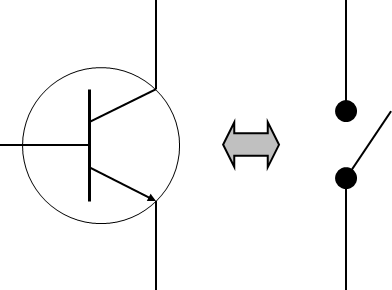
\includegraphics[width=.6\textwidth]{images/transistor_bl}

\textit{Transistor bloqué}

\footnotesize{\textit{Interrupteur ouvert)}}

\footnotesize{\textit{Le courant ne passe pas}}

\footnotesize{\textit{État logique : 0}}

\end{center}
\end{minipage}\hfill
\begin{minipage}[c]{.45\linewidth}
\begin{center}
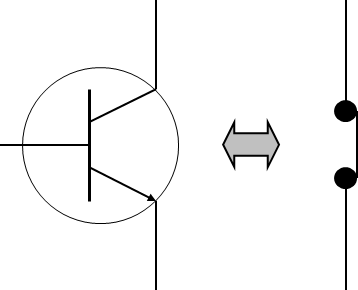
\includegraphics[width=.6\textwidth]{images/transistor_ouv}

\textit{Transistor saturé}

\footnotesize{\textit{(interrupteur fermé)}}

\footnotesize{\textit{Le courant passe}}

\footnotesize{\textit{État logique : 1}}

\end{center}
\end{minipage}

\begin{minipage}[c]{.45\linewidth}
Ces deux états logiques, conventionnellement notés 0 et 1, déterminent cette logique binaire correspondant (de manière un peu « réductrice ») à deux niveaux électriques.

Les informations traitées par les ordinateurs sont de différents types (nombres, instructions, textes, images, sons) mais elles sont toujours représentées en binaire aussi bien en interne, comme on vient de le voir, que sur les « fils » permettant de faire circuler l'information entre les composants de l'ordinateur. 

\end{minipage}\hfill
\begin{minipage}[c]{.45\linewidth}
\begin{center}
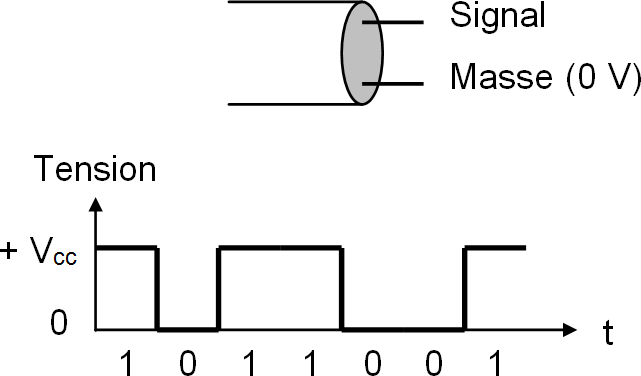
\includegraphics[width=.9\textwidth]{images/transmission_classique}
\end{center}
\end{minipage}



\begin{rem}
On se limitera ici au codage des données numériques (nombres entiers naturels et nombres à virgule).
\end{rem}

\subsection{Notion de mot}

\begin{defi}
\textbf{Mot} -- \textit{Word}

Ensemble de bits de longueur fixe. 

Suivant le type de processeur, les mots peuvent avoir 32, 64 ou 128 bits pour les processeurs Intel Itanium.
\end{defi}

%\begin{center}
%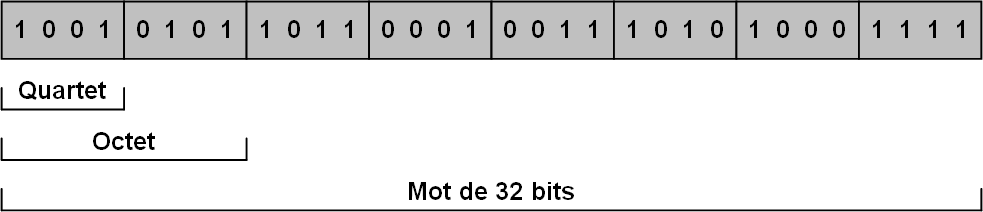
\includegraphics[width=.9\textwidth]{images/mots}
%\end{center}

\footnotesize{
\begin{center}
\begin{tabular}{|cccc|cccc|cccc|cccc|cccc|cccc|cccc|cccc|}
\hline
1&0&0&1&0&1&0&1&1&0&1&1&0&0&0&1&0&0&1&1&1&0&1&0&1&0&0&0&1&1&1&1\\
\hline
\multicolumn{32}{c}{} \\
\multicolumn{4}{|c|}{Quartet} & \multicolumn{28}{c}{} \\
\cline{0-3}
\multicolumn{32}{c}{} \\
\multicolumn{8}{|c|}{Octet} & \multicolumn{24}{c}{} \\
\cline{0-7}
\multicolumn{32}{c}{} \\
\multicolumn{32}{|c|}{Mot de 32 bits} \\
\hline
\end{tabular}
\end{center}
}
\begin{rem}
\textit{byte} est la traduction anglaise du mot octet. En conséquence, un \textit{byte} équivaut à une séquence de 8 bits.
\end{rem}


\subsection{Notion de pondération}
\begin{defi}
\textbf{Écriture d'un nombre dans une base}

Dans un système de numération en base $B$, un nombre noté $N_B$ peut s'écrire sous la forme :
$$
N_B = \sum\limits_{k=0}^{n} a_k \cdot B^k
$$

s'écrit symboliquement sous la forme : 
$$
N_B = \underbrace{\left(a_n a_{n-1} \cdot \cdot \cdot a_2 a_1 a_0\right)_B}_{n+1 \text{ chiffres}}
$$
On note : 
\begin{itemize}
\item $B$ : la base ou nombre de chiffres différents qu'utilise le système de numération;
\item $a_k$ : chiffre de rang $k$;
\item $B^k$ la pondération associée à $a_k$.
\end{itemize}

\end{defi}

\begin{exemple}
$$247_{(10)} = 2\cdot 10^2 + 4\cdot 10^1 + 7\cdot 10^0$$
On appelle : 
\begin{itemize}
\item $2$ est appelé digit de poids fort (\textit{most significant digit});
\item $7$ est appelé digit de poids faible (\textit{least significant digit});
\end{itemize}

$$
1001_2 = 1\cdot 2^{11_2} + 0\cdot 2^{10_2} + 0\cdot 2^{1_2} + 1\cdot 2^{0_2} 
= 1\cdot 2^{3_{10}} + 0\cdot 2^{2_{10}} + 0\cdot 2^{1_{10}} + 1\cdot 2^{0_{10}}
$$
\end{exemple}

\begin{rem}
Par la suite, lorsque la base n'est pas précisée, on se considèrera dans le système décimal. 


\end{rem}

\subsection{Les systèmes de numération}
\subsubsection{Système décimal}
Le système décimal est le système universellement utilisé. C'est la base de référence, ce qui signifie qu'un nombre est de manière implicite écrite en décimal, dès ors qu'il est écrit dans précision de base. 

\subsubsection{Système binaire}

C'est la base de numération couramment utilisée en électronique ou informatique. C'est un système en base 2, l'écriture des nombres est donc composée des caractères de 0 et 1. 

\begin{exemple}

\begin{minipage}[c]{.4\linewidth}
En binaire on compte de la manière suivante : 
\begin{center}
\begin{tabular}{|c|c|}
\hline
Base 10 & Base 2 \\
\hline \hline
0 & 0000 \\ \hline
1 & 0001 \\ \hline
2 & 0010 \\ \hline
3 & 0011 \\ \hline
4 & 0100 \\ \hline
\end{tabular}
\end{center}
\end{minipage}% \hfill
%\begin{minipage}{.57\linewidth}
\textit{Convertir $\left(11011001\right)_2$ en base 10.}
%\end{minipage}
\end{exemple}

\subsubsection{Système hexadécimal}
Ce système à base 16 est le plus utilisé en électronique numérique car il permet une représentation compacte ce qui, dans les systèmes actuels à grande capacité mémoire, est un avantage non négligeable.

\begin{exemple}
\begin{minipage}[c]{.4\linewidth}
En hexadécimal on compte de la manière suivante : 
\begin{center}
\begin{tabular}{|c|c||c|c|}
\hline
Base 10 & Base 16 & Base 10 & Base 16\\
\hline \hline
0 & 00 & 10 & 0A \\ \hline
1 & 01 & 11 & 0B \\ \hline
2 & 02 & 12 & 0C \\ \hline
3 & 03 & 13 & 0D \\ \hline
4 & 04 & 14 & 0E \\ \hline
5 & 05 & 15 & 0F \\ \hline
6 & 06 & 16 & 10\\ \hline
7 & 07 & 17 & 11 \\ \hline
8 & 08 & 18 & 12 \\ \hline
9 & 09 & 19 & 13 \\ \hline
\end{tabular}
\end{center}
\end{minipage}% \hfill
\begin{minipage}{.57\linewidth}
$$\left(2BC5 \right)_{16} = 11 205$$
\end{minipage}
\end{exemple}

\section{Représentation des nombres entiers naturels -- $\mathbb{N}$}

\subsection{De la base k à la base 10}
%\ifthenelse{\boolean{xp}}{
%}{
\begin{savoir}
\textbf{Savoir-Faire :}
Représenter en base dix un entier naturel donné en base $k$.

Pour trouver la représentation en base dix d’un entier naturel donné en base $k$, on
utilise le fait qu’en base $k$, le chiffre le plus à droite représente les unités, le précédent
les paquets de k, le précédent les paquets de $k \cdot k = k^2$, le précédent les paquets de
$k \cdot k \cdot k = k^3$, \textit{etc}.
\end{savoir}
%}


\begin{exemple}
Conversion du nombre $\left(10101\right)_2$ :
\begin{eqnarray*}
\left(10101\right)_2 &=& 1\cdot 2^{4}+0\cdot 2^{3}+1\cdot 2^{2}+0\cdot 2^{1}+1\cdot 2^{0} \\
 & = & 16 + 0 + 4 + 0  + 1\\
 & = & 21\\
\end{eqnarray*}
\end{exemple}

\begin{exemple}
Convertir $(100101)_2$ et $(2C5A)_{16}$ en base 10. 
\vspace{5cm}
\end{exemple}
\subsection{De la base 10 vers la base k}

\ifthenelse{\boolean{xp}}{
}{
\begin{savoir}
SAVOIR-FAIRE Représenter en base k un entier naturel donné en base dix.

Pour écrire les entiers naturels en base k, on a besoin de k chiffres. Quand on a n
objets, on les groupe par paquets de k, puis on groupe ces paquets en paquets de k
paquets, etc. Autrement dit, on fait une succession de divisions par k, jusqu’à obtenir
un quotient égal à 0.
\end{savoir}
}

\subsubsection{Méthode des divisions successives}
\begin{methode}
\textbf{Divisions successives}

On note $N_{10} = a_n\cdot k^n + a_{n-1}\cdot k^{n-1}+ ... +a_1\cdot k^1 + a_0\cdot k^0 = a_n a_{n-1}...a_1 a_0$

\begin{enumerate}
\item Calcul de la division de $N_{10}$ par k.
\begin{itemize}
\item Le reste de la division correspond au terme $a_0$.
\end{itemize}
\item Le dividende de la division est divisé par k.
\begin{itemize}
\item Le reste de la division correspond au terme $a_1$.
\end{itemize}
\item ....
\end{enumerate}

La division s'arrête lorsque le dividende est nul.
\end{methode}

\begin{exemple}
\textit{Conversion de $247_{10}$ en binaire.}

\begin{center}
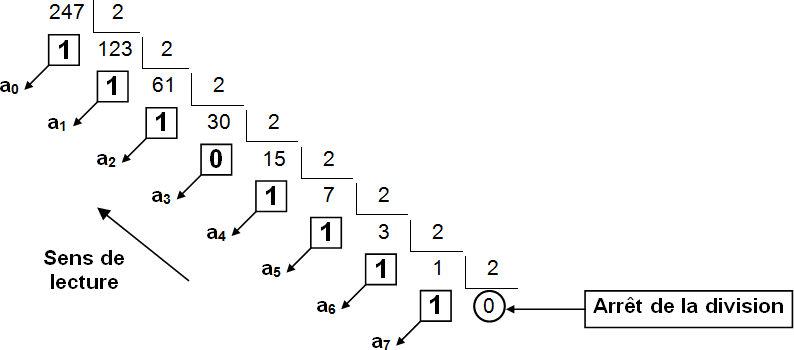
\includegraphics[width=.7\textwidth]{images/conversion_binaire}
\end{center}

Ainsi $(247)_{(10)}=(11110111)_{(2)}$.

\textit{Convertir 247 en base 16.}

\vspace{4cm}
\end{exemple}

\subsubsection{Méthode de la plus grande puissance}
\begin{methode}

Elle consiste à retrancher du nombre initial la plus grande puissance de k possible et ainsi de suite dans l’ordre décroissant des puissances. Si on peut retirer la puissance de k concernée, on note 1 sinon on note 0 et on continue de la sorte jusqu’à la plus petite puissance de k possible soit $k^0$ pour des entiers naturels.
\end{methode}

\begin{exemple}
\textit{Conversion de $247_{10}$ en binaire.}

\begin{center}
\begin{tabular}{llllllll}
 & & & $\diamond$ & & $\triangle$ & & \\
De & 247 & on peut retirer & 0 & fois & 256. &Il reste & 247. \\
De & 247 & on peut retirer & 1 & fois & 128. &Il reste & 119. \\
De & 119 & on peut retirer & 1 & fois & 64. &Il reste & 55. \\
De & 55 & on peut retirer & 1 & fois & 32. &Il reste & 23. \\
De & 23 & on peut retirer & 1 & fois & 16. &Il reste & 7. \\
De & 7 & on peut retirer & 0 & fois & 8. &Il reste & 7. \\
De & 7 & on peut retirer & 1 & fois & 4. &Il reste & 3. \\
De & 3 & on peut retirer & 1 & fois & 2. &Il reste & 1. \\
De & 1 & on peut retirer & 1 & fois & 1. &Il reste & 0. \\
\end{tabular}
\end{center}

$\diamond$ : lors d'une conversion en base 2, on n'utilise dans cette colonne que des 0 ou des 1. 

$\triangle$ : lors d'une conversion en base 2, on n'utilise dans cette colonne que des puissances de 2 ($2^n$).

Les valeurs binaires sont lues de haut en bas. On obtient bien le même résultat : $(247)_{(10)}=(11110111)_{(2)}$.

\textit{Convertir 247 en base 16.}

\vspace{3cm}

\end{exemple}

\ifthenelse{\boolean{xp}}{
}{
\begin{exercice}
Exercice: Trouver la représentation en base cinq de 58.
\end{exercice}
}

\ifthenelse{\boolean{xp}}{
}{
\begin{exercice}
Exercice: Trouver la représentation en base seize du nombre 1207.
\end{exercice}
}







\subsection{Capacités de la représentation}

Les limites du codage des nombres entiers naturels sont dues à la longueur du mot binaire nécessaire pour les coder. 


\begin{resultat}
Si un mot est codé sur $n$ bits, on peut représenter un entier naturel compris entre 0 et $2^n-1$, soit $2^n$ valeurs possibles. 
\end{resultat}

\begin{exemple}
Si les mots sont codés sur un octet (8 bits), on peut compter de 0 à $2^8-1$, c'est-à-dire de 0 à 255. 

\begin{center}
\begin{tabular}{|c|c|c|}
\hline 
\textbf{Bits} & \textbf{Nombre de valeurs} & \textbf{de 0 à ...} \\\hline
4   & 16 & 15 \\ \hline
8   & 256 & 255 \\ \hline
16 & 65 536 & 65 535 \\ \hline
32 & 4,29... milliards &  4,29... milliards \\ \hline
64 & $1,84... 10^{19}$ & $1,84... 10^{19}$ \\ \hline

\end{tabular}
\end{center}
\end{exemple}

\begin{rem}
\textbf{Dépassement de capacité} -- \textit{Overflow}

Le résultat de l'addition de deux nombres codés sur le même nombre de bit n'est pas toujours possible car le résultat pourrait demander des bits supplémentaires. 

En effet, considérons un système où les mots sont codés sur un octet. Calculons $247_{(10)} + 53_{(10)}$
$$
247_{(10)} + 53_{(10)} = 300_{(10)} = 1\underbrace{00101100}_{\text{octet retenu}}
$$

Ainsi le résultat retenu est $001011100_{(2)}=44_{(10)}$ au lieu de $300_{(10)}$. 

On parle alors de dépassement de capacité (\textit{overflow} en anglais). Sur certains ordinateurs, les calculs continuent. Sur d’autres, une erreur est signalée, d’une façon différente d’un constructeur à l’autre.
\end{rem}

\begin{resultat}
\textbf{Addition en binaire}

En binaire, l'addition peut être considérée ainsi :
$$\left\{\begin{array}{l}
0_2+0_2=0_2\\
1_2+0_2=1_2\\
0_2+1_2=1_2\\
1_2+1_2=10_2
\end{array}
\right.$$

On en déduit rapidement que l'addition en binaire s'effectuera sur le même principe que l'addition en écriture décimale, à ceci près que la retenue se produit dès qu'on arrive à 2 (au lieu de 10).
\end{resultat}
\begin{exemple}
\textit{Somme de deux nombres binaires}

\begin{center}
\begin{tabular}{p{2cm}|c|c|c|c|c|c|c|c|c|}
\multicolumn{1}{c}{}  & 
\multicolumn{1}{c}{1} & 
\multicolumn{1}{c}{1} & 
\multicolumn{1}{c}{1} & 
\multicolumn{1}{c}{1} & 
\multicolumn{1}{c}{0} & 
\multicolumn{1}{c}{1} & 
\multicolumn{1}{c}{1} & 
\multicolumn{1}{c}{1} &
\multicolumn{1}{c}{}  \\
\cline{3-10}
\multicolumn{1}{c}{$247_{(10)} \quad \rightarrow $} &  & 1 & 1 & 1 & 1 & 0 & 1 & 1 & 1 \\
\cline{3-10}
\multicolumn{1}{c}{$53_{(10)} \quad \rightarrow $} & + & 0 & 0 & 1 & 1 & 0 & 1 & 0 & 1 \\
\cline{3-10}
\multicolumn{10}{c}{} \\
\cline{2-10}
\multicolumn{10}{c}{} \\
\cline{2-10}
& 1 & 0 & 0 & 1 & 0 & 1 & 1 & 0 & 0 \\
\cline{2-10}
\end{tabular}
\end{center}

\end{exemple}

\section{Codage pondéré des entiers relatifs -- $\mathbb{Z}$}
\ifthenelse{\boolean{prof}}{}{
\begin{savoir}
Représenter en binaire sur $n$ bits un entier relatif donné en décimal.

Si l’entier relatif $x$ est positif ou nul, on le représente comme l’entier naturel $x$. S’il est
strictement négatif, on le représente comme l’entier naturel $x + 2^n$.
\end{savoir}

\begin{savoir}
Trouver la représentation décimale d’un entier relatif donné en binaire sur n bits.

Si cet entier relatif est donné par le mot m, on commence par calculer l’entier naturel
p représenté par ce mot. Si p est strictement inférieur à $2^n-1$, c’est l’entier relatif
représenté, s’il est supérieur ou égal à $2^n-1$, l’entier relatif représenté est $p-2^n$.
\end{savoir}
}

\subsection{Première approche}
La première solution envisageable pour représenter un entier relatif est de dédier un bit pour le codage du signe puis de représenter sur les autres bits la valeur absolue. La convention retenue impose de mettre le bit de poids fort à 0 pour repérer un nombre positif et à 1 pour un nombre négatif. 

On parle de nombres signés quand on utilise cette convention.

\begin{exemple}
\textit{Conversion en binaire sur un octet des nombres $+81_{(10)}$ et $-81_{(10)}$.}


\begin{center}
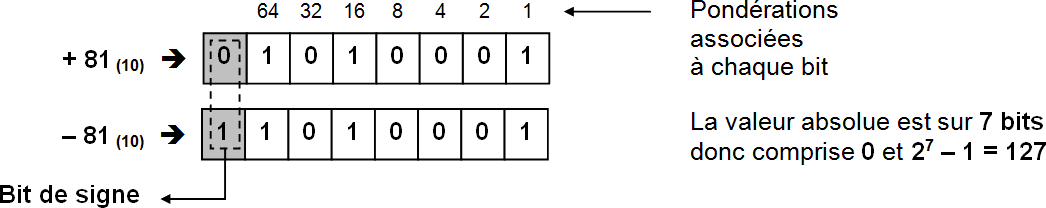
\includegraphics[width=.7\textwidth]{images/entier_relatif}
\end{center}

\end{exemple}

\begin{rem}
\textit{Inconvénients : addition binaire de $+81_{(10)}$ et $-81_{(10)}$}
Cette représentation des nombres signés, si elle est facile à mettre en œuvre, ne permet pas d’utiliser les règles de l’addition binaire pour obtenir un résultat correct. De plus, il y a deux zéros, l’un positif, l’autre négatif.

\begin{center}
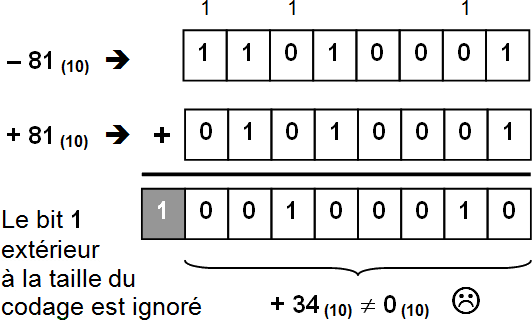
\includegraphics[width=.35\textwidth]{images/entier_relatif_2}
\end{center}

Du fait des problèmes d’arithmétique qu’il pose, ce codage est rarement utilisé.

Cet inconvénient est résolu par l’usage d’une autre forme de représentation des nombres négatifs dit représentation en complément ou représentation sous forme complémentée.

\end{rem}

\subsection{Codage des entiers relatifs en complément à deux}
Les règles suivantes sont adoptées par la majeure partie des constructeurs.



\textit{Nombre entier relatif sur un octet (n = 8 bits)}

\begin{center}
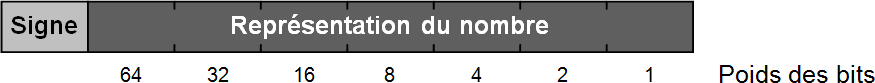
\includegraphics[width=.7\textwidth]{images/entier_relatif_3}
\end{center}
\begin{itemize}
\item Signe = 1 : Nombre négatif 
\item Signe = 0 : Nombre positif
\item La valeur zéro est considérée comme un nombre positif.
\item Les nombres positifs sont représentés sous leur forme binaire.
\item Leur valeur est codée sur n – 1 = 8 – 1 = 7 bits (et non 8 bits).
\item Les nombres négatifs sont représentés sous leur forme complément à deux.
\end{itemize}

\subsubsection{Première méthode pour l’obtention du complément à deux d’un nombre négatif}

\begin{methode}
Pour représenter l’opposé d’un nombre positif par son complément à deux, on inverse les bits 0 et 1 et on ajoute 1 au mot binaire obtenu.
\end{methode}

\begin{exemple}
\textit{Complément à deux du nombre $-81_{(10)}$ sur un octet.}

\begin{center}
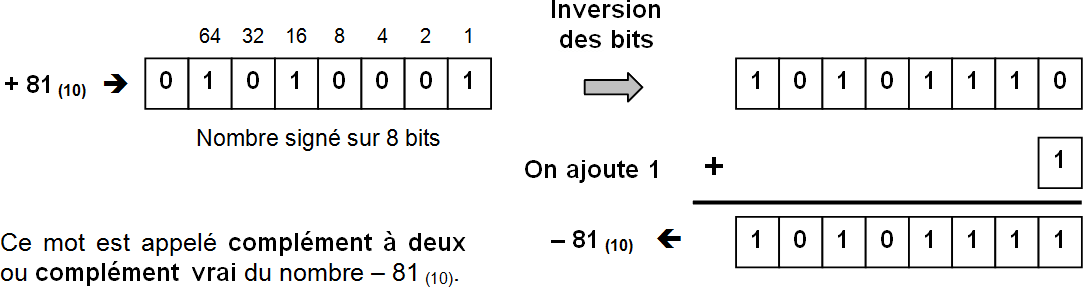
\includegraphics[width=.7\textwidth]{images/complement_2}
\end{center}

\end{exemple}

\subsubsection{Seconde méthode pour l’obtention du complément à deux d’un nombre négatif}

\begin{methode}
On représente un entier relatif $a \geq 0$ comme l’entier naturel $a$.

On représente un entier relatif $a < 0$ comme l’entier naturel $a + 2^n$.

\end{methode}

\begin{exemple}
\textit{Complément à deux du nombre $-81_{(10)}$ sur un octet.}

\textit{Vérification de $-81_{(10)} + 81_{(10)} = 0_{(10)}$.}

\begin{center}
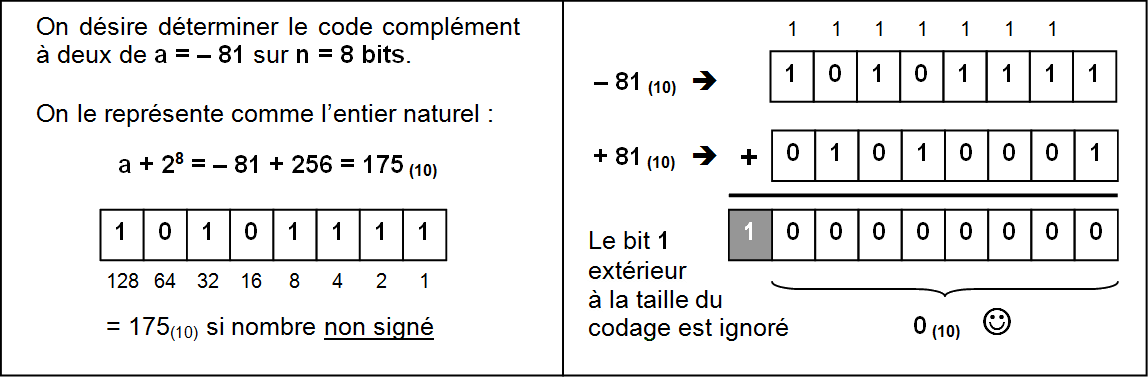
\includegraphics[width=.7\textwidth]{images/complement_2_2}
\end{center}

\end{exemple}


\begin{exercice}
Exercice: Trouver les représentations binaires sur huit bits des entiers relatifs 0 et -128.
\end{exercice}

\begin{exercice}
Exercice: Trouver les représentations décimales des entiers relatifs dont les représentations
binaires sur huit bits sont 00010111 et 10001100.
\end{exercice}
\subsection{Retour en décimal}

\begin{exemple}
Trouver la représentation décimale des entiers relatifs dont les représentations binaires sur huit bits sont $01010101$ et $10101010$.

\vspace{4cm}
\end{exemple}


\subsection{Limites de la représentation}
\begin{center}
\begin{tabular}{|c|c|c|}
\hline
Taille du mot & Nombre de bits & Valeurs décimales \\
\hline
$n$ bits & 1 bit de signe & 0 à $+2^{n-1}-1$ \\
$n$ bits & n-1 bits de valeur & -1 à $-2^{n-1}$ \\ \hline
$8$ bits & 1 bit de signe & 0 à + 127 \\
$8$ bits & 7 bits de valeur & -1 à -128 \\ \hline
$16$ bits & 1 bit de signe & 0 à +32 767 \\
$16$ bits & 15 bits de valeur & -1 à -32 768 \\ \hline
$32$ bits & 1 bit de signe & 0 à +2 147 483 647 \\
$32$ bits & 31 bits de valeur & -1 à -2 147 483 648 \\ \hline
\end{tabular}
\end{center}

Les limites du codage des entiers relatifs sont principalement dus au dépassement de capacité (overflow) lors d’un calcul. Une addition de deux nombres positifs ou négatifs peut entraîner un dépassement de capacité, celui-ci peut être détecté en regardant le signe du résultat par rapport au signe des deux opérandes (deux nombres positifs donnent un résultat négatif et réciproquement).

\begin{rem}
Dans les versions Python 2.x
Lorsque la capacité des entiers machine (32 ou 64 bits) a été dépassée, les nombres sont
suivis du marqueur L, qui explicite qu’on passe dans un autre type appelé long. La dernière
ligne de l’exemple précédent affiche donc plutôt
\begin{py}
\begin{python}[H]
In [4]: a*a*a*a
Out[4]: 4569760000L
\end{python}
\end{py}
En Python 3.x, les types int et long sont fusionnés, et à toutes fins utiles les entiers sont
toujours de taille illimitée. Le marqueur L n’est plus utilisé.
\end{rem}

\begin{exercice}
Représenter les entiers relatifs 99 et 57 en binaire sur huit bits. Ajouter les deux nombres
binaires obtenus. Quel est l’entier relatif obtenu ? Pourquoi est-il négatif ?

Trouver la représentation décimale des entiers relatifs dont les représentations binaires sur
huit bits sont 01010101 et 10101010.

Quels entiers relatifs peut-on représenter avec des mots de 8 bits ? Combien sont-ils ?
Même questions avec des mots de 16 bits, 32 bits et 64 bits.

(À réaliser dans une version Python 2.x)
À l’aide de la calculatrice Python, déterminer le plus grand entier représentable par le type int sur votre
machine. Vérifiez si votre machine fonctionne en 32 bits ou en 64 bits et calculez la valeur théorique de
ce plus grand entier pour vérifier votre réponse.
\end{exercice}

\subsection{Notation hexadécimale}

Pour un nombre donné, il faut beaucoup de chiffres en binaire. Dès lors qu’on manipule de grandes séries binaires, on a besoin d’une notation plus concise que le binaire telle que le passage entre elle et le binaire soit très facile. La solution est de faire appel à une base qui soit une puissance de 2. Aujourd’hui, on emploie universellement l’hexadécimal (base $16 = 2^4$). 

En notation hexadécimale, on utilise un alphabet comportant 16 symboles (10 chiffres et 6 lettres) : 

0    1    2    3    4    5    6    7    8    9    A    B    C    D    E    F

\begin{methode}
Pour convertir de binaire à hexadécimal, on regroupe les bits par quartet (en ajoutant des 0 à gauche si nécessaire) et on remplace chaque quartet par le symbole hexadécimal correspondant. D’hexadécimal à binaire, on effectue l’opération inverse.
\end{methode}

\subsubsection*{Table de correspondance entre nombres hexadécimaux, décimaux et binaires}


\footnotesize{\begin{center}
\begin{tabular}{|c|c|c|c|c|c|c|c|c|c|c|c|c|c|c|c|c|}
\hline 
$N_{(10)}$ & 
0	&
1	&
2	&
3	&
4	&
5	&
6	&
7	&
8	&
9	&
10	&
11	&
12	&
13	&
14	&
15 \\
\hline
$N_{(16)}$ &
0	&
1	&
2	&
3	&
4	&
5	&
6	&
7	&
8	&
9	&
A	&
B	&
C	&
D	&
E	&
F\\
\hline
$N_{(2)}$ & 
 0000	&
 0001	&
 0010	&
 0011	&
 0100	&
 0101	&
 0110	&
 0111	&
 1000	&
 1001	&
 1010	&
 1011	&
 1100	&
 1101	&
 1110	&
 1111\\
\hline
\end{tabular}
\end{center}}

\begin{exemple}
$$
3863_{(10)} = 
\underbrace{1111}_{F} \quad 
\underbrace{0001}_{1} \quad 
\underbrace{0111}_{7} \quad_{(2)}=F17_{(16)}
$$
%On note aussi $3863_{(10)} = 0xF17$.

\end{exemple}
\normalsize
\begin{rem}
La représentation des valeurs sous format hexadécimal ne se traduit pas visuellement par la présence de l’indice $_{(16)}$ derrière la valeur. On utilise parfois la lettre H mais on notera le plus souvent la base 16 par la présence d’un $0x$ (comme heXadécimal) devant le nombre. 
$F17_{(16)}$, $F17H$ ou $0xF17$ sont des représentations valides d’une même valeur hexadécimale.

\end{rem}






\begin{thebibliography}{2}
\bibitem{cf}{Christophe François, Représentation de l'information, représentation des nombres.}
%\bibitem{zero}{Apprenez à programmer en Python \url{http://www.siteduzero.com/}.}
\bibitem{Manfred}{Manfred GILLI, METHODES NUMERIQUES, Département d’économétrie
Université de Genève, 2006.}
\end{thebibliography}
\end{document}
